% The global state, field by field (generic_model.v, state_type), shaded by the state
% equivalence: public (dark) or private (white) to the attacker.  Laid out like the
% columns of fig:io: a framed column with its operator in the title, a nested sum or
% product side by side within a row.  proof.tex inputs this file in the state equivalence.
\begin{figure}[t]
\centering
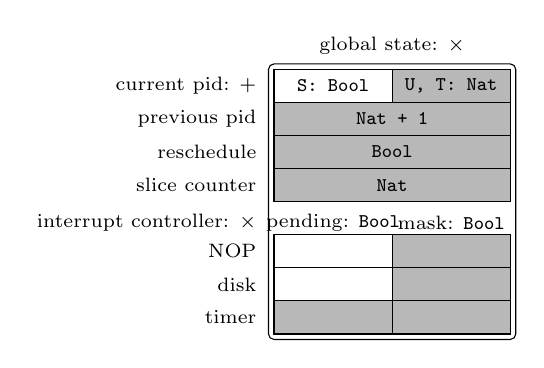
\begin{tikzpicture}[font=\scriptsize,
  c/.style={draw, minimum height=0.42cm, inner sep=0pt, font=\ttfamily\scriptsize},
  pub/.style={c, fill=black!28}, priv/.style={c, fill=white}]
% fields, one row each, cells spanning x = 0 .. 3.0
\node[anchor=east] at (-0.1,0) {current pid: $+$};
\node[priv, minimum width=1.5cm] at (0.75,0) {S: Bool};
\node[pub, minimum width=1.5cm] at (2.25,0) {U, T: Nat};
\foreach \y/\l/\t in {-0.42/previous pid/Nat + 1, -0.84/reschedule/Bool,
                      -1.26/slice counter/Nat}
  {\node[anchor=east] at (-0.1,\y) {\l};
   \node[pub, minimum width=3.0cm] at (1.5,\y) {\t};}
% the interrupt controller: one entry per handler, each pending x mask
\node[anchor=east] at (-0.1,-1.74) {interrupt controller: $\times$};
\node at (0.75,-1.74) {pending: \texttt{Bool}};
\node at (2.25,-1.74) {mask: \texttt{Bool}};
\foreach \y/\l/\p in {-2.1/NOP/priv, -2.52/disk/priv, -2.94/timer/pub}
  {\node[anchor=east] at (-0.1,\y) {\l};
   \node[\p, minimum width=1.5cm] at (0.75,\y) {};
   \node[pub, minimum width=1.5cm] at (2.25,\y) {};}
\draw[rounded corners=2pt] (-0.07,-3.22) rectangle (3.07,0.28);
\node[anchor=south] at (1.5,0.28) {global state: $\times$};
\end{tikzpicture}
\caption{The global state \changed{of \cref{sec:global-state}}, field by field,
  \changed{shaded as in \cref{fig:io} by the state equivalence}. The current pid is a sum: its \texttt{inl}
  side holds a secret handler (an S step), a \texttt{Bool} saying which one, and
  its \texttt{inr} side the number of any other process (U or T). Its
  equivalence is $\privvis + \pubeq$ (\cref{def:formers}), so
  the tag is public: whether a secret handler runs is public; which one runs is private.
  So are the pending bits of the NOP and disk handlers. Every other field,
  \texttt{None} included, is public.}
\label{fig:state}
\end{figure}
